\section{Einleitung}
In diesem Proseminar sehen wir uns eine Einführung in TensorFlow, Keras und PyTorch an. 
Hierbei handelt es sich um die relevantesten Machine Learning Frameworks zur Zeit. 
TensorFlow wird seit 2015 für den Google-internen Bedarf entwickelt und 
wurde 2017 unter einer Open-Source Lizenz veröffentlicht. 
Keras bot ursprünglich eine Schnittstelle für verschiedene Machine Learning Backends an, welche 
einem das Programmieren durch High-Level Funktionen vereinfachen soll. 
Seit dem Release von Keras 2.4 wurde die Unterstützung verschiedener 
Backends eingestellt und Keras ist zu einem Teil der TensorFlow Core API geworden. 
PyTorch wurde 2016 von Facebook veröffentlicht. Dieses Framework basiert auf 
der Lua-Bibliothek Torch, welche bereits seit 2002 existiert.

\section{PyTorch}
\subsection{Daten laden und präparieren}
Wenn man ein neuronales Netz erstellen und einsetzen möchte, kann man dies in grob 
drei Schritte unterteilen: 
\begin{enumerate}
    \item Daten einlesen und vorverarbeiten
    \item Modell erstellen
    \item Modell trainieren
\end{enumerate}

Möchte man populäre, weit verbreitete Datensätze für sein Modell verwenden, bietet sich 
\code{torchvision.datasets}\footnote{\url{https://pytorch.org/vision/stable/datasets.html}} 
an. Dort gibt es viele bekannte Datensätze für die verschiedensten Probleme 
wie z.~B. MNIST\footnote{70000 handgeschriebene Ziffern: \url{http://yann.lecun.com/exdb/mnist}} für Ziffernerkennung, 
ImageNet\footnote{1,4 Millionen Bilder, 1000 verschiedene Klassen: \url{http://image-net.org}} für Bildklassifizierung oder 
Cityscapes\footnote{Videos aus dem Straßenverkehr: \url{https://www.cityscapes-dataset.com}} 
zur Klassifizierung von Elementen im Straßenverkehr. 

\lstinputlisting[label=py:pytorch-load-data, language=Python, caption=MNIST Datensatz mit TorchVision herunterladen.]{code/load-data-pytorch.py}
In Listing \ref{py:pytorch-load-data} sehen wir am Beispiel MNIST, wie wir so einen Datensatz herunterladen 
und für unser Modell präparieren können. Hierfür erstellen wir einfach eine 
Instanz der Klasse \code{datasets.MNIST} und können dort noch ein paar Optionen angeben. 
Wichtig für das neuronale Netz ist die Option \code{transform}, mit welcher wir 
die Daten vorher noch transformieren können. In unserem Beispiel konvertieren wir die 
Daten in einen Tensor und führen danach \code{torch.flatten} aus, was dazu führt, dass 
aus einem \(28 \times 28\)-Tensor ein \(784\)-Tensor wird.
Das benötigen wir, da Fully Connected Neural Networks nicht 
mit zwei Dimensionalen Tensoren umgehen können. 
Hier könnte man allerdings auch noch viele andere Vorverarbeitungsschritte machen: 
PCA\footnote{\url{https://en.wikipedia.org/wiki/Principal_component_analysis}}, die Pixelwerte auf dem Bild normalisieren, etc.

Sind die Daten nun heruntergeladen, können sie an einen \code{DataLoader} gegeben werden. 
Dieser liest die Daten ein, teilt sie in Batches auf (damit der Speicher nicht überfüllt wird) 
und kann die Daten außerdem noch mischen, damit kein Bias entsteht.

\subsection{Modellerstellung}
Haben wir die nötigen Daten geladen, ist es nun an der Zeit, das Modell zu erstellen. 
Ich zeige das ganze hier der Einfachheit halber an einem Fully Connected Neural Network 
mit einem Hidden Layer mit 64 Knoten, komplexere Modelle funktionieren allerdings relativ ähnlich. 

\begin{figure}[htbp]
    \centering
    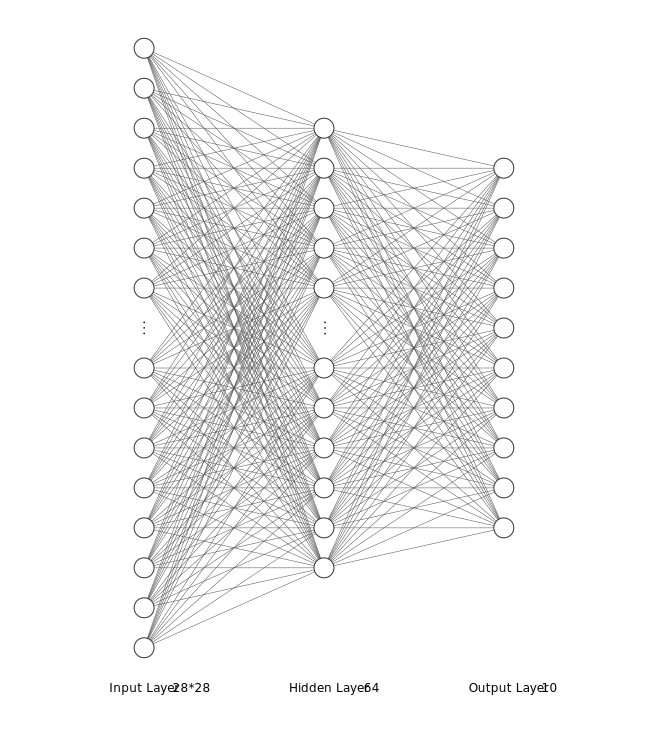
\includegraphics[width=.6\textwidth]{figures/fcnn-28x28-64-10}
    \caption{Fully Connected Neural Network.}
    \label{fig:fcnn}
\end{figure}

\lstinputlisting[label=py:pytorch-model-creation, language=Python, caption=Modellerstellung in PyTorch.]{code/create-model-pytorch.py}
In Listing \ref{py:pytorch-model-creation} sehen wir nun, wie das ganze in PyTorch realisiert wird. 
Wir erben von der Klasse \code{torch.nn.Module} und müssen nur zwei Sachen implementieren: 
den Konstruktor und die Forward-Funktion.
Im Konstuktor erstellen wir zwei Layer. Auch wenn es in Abbildung \ref{fig:fcnn} 
so aussieht als hätten wir drei Ebenen, sind die Ebenen, die wir implementieren, 
die Verbindungslinien zwischen den Knoten, von denen es nur zwei gibt: 
die erste Ebene verbindet das Input Layer (\(28 \cdot 28\) Pixel \(\Rightarrow 28 \cdot 28\) Knoten) 
mit dem Hidden Layer (\(64\) Knoten), die zweite Ebene verbindet die \(64\) Knoten des Hidden Layers
mit dem Output Layer (\(10\) verschiedene Ziffern \(\Rightarrow 10\) Klassen).
In der Forward-Methode müssen wir nur implementieren, was die Ausgabe des 
neuronalen Netzes sein soll, wenn wir eine Eingabe \(x\) in das Netzwerk geben. 
Wir wenden natürlich das erste Layer auf \(x\) an, schicken es ins Hidden Layer, 
darauf die Aktivierungsfunktion und senden diese Daten dann über \code{fc2} an das Output Layer.
Damit wir zum Schluss auch noch auf eine Wahrscheinlichkeitsverteilung kommen, 
wenden wir auf die letzte Ebene noch die Softmax-Aktivierungsfunktion \(\sigma(z)_j = \frac{\exp(z_j)}{\sum_{i} \exp(z_i)}\) an.

\subsection{Modell trainieren}
Nachdem wir alle notwendigen Schritte vollführt haben, ist es jetzt an der Zeit, das Modell zu trainieren. 
Wir werden hier als Optimierungsalgorithmus Stochastic Gradient Descent verwenden und als Loss-Funktion 
wie üblich bei Klassifizierungsproblemen Cross-Entropy-Loss. 
Um über die Daten zu iterieren, verwenden wir den oben definierten 
\code{DataLoader}, welcher uns automatisch gemischte sowie gut portionierte Daten 
gibt, auf denen wir nun Gradient Descent ausführen können. 
Mit \code{optimizer.zero\_grad} weisen wir den Optimierungsalgorithmus darauf hin, 
dass der Gradient auf Null gesetzt werden soll. Das müssen wir in jedem Schritt machen, 
da PyTorch die Gradienten sonst aufaddieren würde, was bei RNNs von Vorteil sein kann, wir hier allerdings nicht benötigen.
Der tatsächliche Optimierungsschritt findet dann in den Zeilen 11-14 statt: 
zuerst der Forward Pass, in welchem die Daten an das neuronale 
Netz gesendet werden und der Loss ausgerechnet wird und danach der Backward Pass, 
in welchem sukzessive der Gradient bezüglich der Gewichte \(\frac{\partial \mathcal{L}}{\partial w}\)
ausgerechnet wird.

\newpage

\lstinputlisting[label=py:pytorch-model-training, language=Python, caption=Modell trainieren in PyTorch.]{code/train-model-pytorch.py}

\section{TensorFlow und Keras}

In TensorFlow können wir die oben beschriebene Vorangehensweise zum Erstellen eines neuronalen Netzes 
relativ analog durchführen. Aus diesem Grund werde ich mich im Folgenden auf die wesentlichen 
Unterschiede zwischen PyTorch und TensorFlow beschränken. 

\subsection{Daten laden und präparieren}

\lstinputlisting[label=py:keras-load-data, language=Python, caption=MNIST Datensatz mit \texttt{keras.datasets} herunterladen.]{code/load-data-tensorflow.py}
Das Analogon zu \code{torchvision.datasets} lautet 
\code{tensorflow.keras.datasets}\footnote{\url{https://www.tensorflow.org/api_docs/python/tf/keras/datasets}}. 
Es gibt allerdings auch noch das Modul \code{tensorflow\_datasets}\footnote{\url{https://www.tensorflow.org/datasets/catalog/overview}}, 
welches einem eine deutlich größere Vielfalt an Datensätzen liefert als das zuerst genannte.
TensorFlow arbeitet mit sogenannten One-Hot-kodierten Tensoren: statt Targets der Form 
\((i)\) für die \(i\)-te Klasse werden Targets der Form \(\begin{pmatrix}
    0 & \cdots & 0 & 1 & 0 \cdots & 0
\end{pmatrix}\) verwendet, wobei die \(1\) an der \(i\)-ten Komponente steht. 
Da die Daten allerdings im ersten Format gegeben sind, müssen wir diese zuerst über \code{tf.one\_hot} umformatieren. 
Die Eingabebilder haben pro Pixel Werte zwischen \(0\) und \(255\). 
Da das neuronale Netz mit normierten Daten zwischen \(0\) und \(1\) besser arbeitet, 
müssen wir diese ebenfalls zuerst anpassen. 

\newpage

\subsection{Modellerstellung}

\lstinputlisting[label=py:keras-model-creation, language=Python, caption=Modellerstellung in TensorFlow.]{code/create-model-tensorflow.py}
Die Modellerstellung ist sehr ähnlich zu PyTorch. Zu beachten ist hier, dass 
wir noch ein \code{Flatten}-Layer hinzugefügt haben. Das ist äquivalent zur 
\code{torch.flatten}-Transformation, die in Listing \ref{py:pytorch-load-data} direkt beim 
Laden des Datensatzes verwendet wird. 
Ob man die Daten bereits beim Laden der Daten auf die gewünschte Form bringt oder das 
erst im neuronalen Netz tut, ist Geschmackssache. 
Die Batch-Size wird in TensorFlow im Gegensatz zu PyTorch erst bei der Modellerstellung 
während \code{model.build} mit der Input-Dimension der Daten angegeben~-- schließlich gibt es 
keinen \code{DataLoader}, der sich explizit um die Portionierung sowie Vorverarbeitung 
der Daten kümmert.

\vspace{2mm}

\subsection{Modell trainieren}
\lstinputlisting[label=py:keras-model-training, language=Python, caption=Modell trainieren in TensorFlow.]{code/train-model-tensorflow.py}
Das Training des neuronalen Netzes geht in TensorFlow ohne explizite Schleifen. 
Wir müssen nur den Optimierungsalgorithmus sowie die Loss-Metrik in \code{model.compile} 
angeben und dann \code{model.fit} mit den jeweiligen Trainings- und 
Validierungsdaten aufrufen. 

%% TODO warum wird die Batch-Size hier erneut verwendet? Warum reicht nicht bereits vorher angegebenes?

\newpage

\subsection{CNN Implementierung}
Wenn man Bilder mit höherer Auflösung als \(28\times 28\) klassifizieren möchte, verwendet man 
meistens Convolutional Neural Networks. Im Folgenden werden wir uns anschauen, wie wir ein solches CNN in Keras 
implementieren können. In Abbildung \ref{fig:cnn} sehen wir die Architektur des CNNs: jeweils drei Convolutional Layer 
mit Max-Pooling Layern dazwischen. Zum Schluss kommt ein Flatten Layer, welches die Daten auf eine Dimension herunterpresst, 
damit wir für die Klassifizierung zum Schluss noch ein letztes FCNN-Layer hinzufügen können.\\
\begin{figure}[htbp]
    \centering
    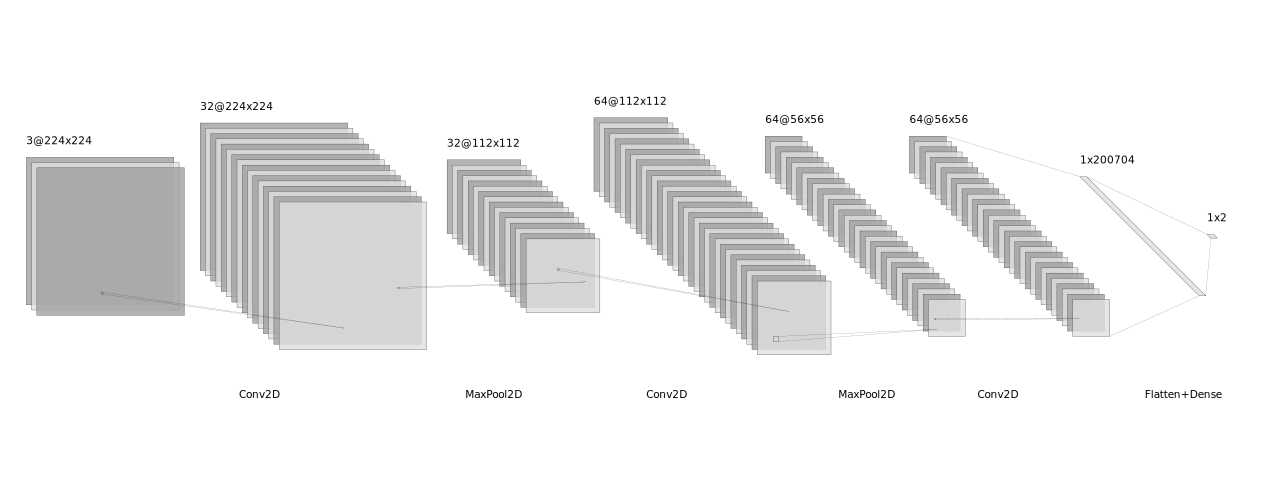
\includegraphics[width=.9\textwidth]{figures/cnn}
    \caption{Convolutional Neural Network.}
    \label{fig:cnn}
\end{figure}\\
In Listing \ref{py:keras-cnn} sehen wir die Implementierung. Da die Daten immer von einem Layer zum 
Folgenden gegeben werden, können wir das \code{Sequential}-Modell aus Keras verwenden. 
Um dieses zu initialisieren, müssen wir ausschließlich ein Array mit den jeweiligen Layern in den 
Konstruktor geben. Die Hyperparameter der jeweiligen Ebenen können wir bei deren Initialisierung angeben.

\lstinputlisting[label=py:keras-cnn, language=Python, caption=CNN Implementierung in Keras.]{code/create-cnn-keras.py}
Das Laden der Testdatensätze sowie das Training des Modells funktionieren analog zu Listing \ref{py:keras-load-data} 
und \ref{py:keras-model-training}. 

\newpage

\subsection{Transfer Learning}
Da man für gute Ergebnisse bei komplexen Problemen neuronale Netze lange trainieren muss, 
ist es heutzutage üblich, sich nicht seine eigenen CNNs selbst zu designen, sondern bereits vortrainierte 
Modelle, welche erwiesenermaßen gut performen, zu verwenden und diese nur leicht abzuändern. \\
In \code{tf.keras.applications}\footnote{\url{https://www.tensorflow.org/api_docs/python/tf/keras/applications}}
finden wir einige bereits vortrainierte Netze. Wir verwenden beispielhaft VGG16\footnote{\url{https://arxiv.org/abs/1409.1556}}, 
der Gewinner des ImageNet Wettbewerbs\footnote{\url{http://www.image-net.org/challenges/LSVRC/}} in 2014. 

\lstinputlisting[label=py:keras-transfer-learning, language=Python, caption=Transfer Learning in Keras.]{code/transfer-learning-keras.py}
In Listing \ref{py:keras-transfer-learning} sehen wir die Implementierung des Transfer Learnings. 
Wir erstellen wie in Listing \ref{py:keras-cnn} ein \code{Sequential}-Modell und fügen nach und nach 
bis auf die letzte alle Ebenen des VGG16-Modells ein. Diese setzen wir auf \gqq{nicht trainierbar} 
und fügen zum Schluss eine eigene Ebene zur Klassifikation ein. Dadurch haben wir nur relativ wenige Parameter, 
die wir effektiv anpassen müssen und kommen so auf eine schnellere Lernperformance.

\subsection{Funktionale Modelle}
Bis jetzt haben wir immer nur sequentielle Implementierungen in Keras betrachtet, wir haben ein \code{Sequential}-Modell erstellt und diesem dann 
die benötigten Ebenen hinzugefügt. Es gibt allerdings noch eine andere Art, wie man Neuronale Netze implementieren kann: durch funktionale Modelle.
Der Output des Netzes lässt sich darstellen als \(y = f_1(f_2(\cdots f_n(x)))\), wobei \(f_i\) die \(i\)-te Ebene ist. 
In Listing~\ref{py:keras-functional-model} sehen wir eine äquivalente funktionale Implementierung zu Listing~\ref{py:keras-cnn}. 
Wir instanziieren die jeweiligen Ebenen wie in der sequentiellen API, geben allerdings die Daten aus dem vorherigen Schritt noch in die Ebene ein. 
Das Modell wird dann durch die Inputs und Outputs definiert. \\
Es ist sinnvoll, sowohl mit der sequentiellen als auch mit der funktionalen API arbeiten zu können, da manche vortrainierten Modelle wie VGG16 in der 
sequentiellen API vorliegen, während andere Modelle wie Xception\footnote{\url{https://www.tensorflow.org/api_docs/python/tf/keras/applications/Xception}}
die funktionale API verwenden.

\newpage

\lstinputlisting[label=py:keras-functional-model, language=Python, caption=Funktionale Modelle in Keras.]{code/functional-keras.py}

\section{Zusammenfassung und Fazit}

Abschließend lässt sich sagen, dass es zwischen TensorFlow und PyTorch heutzutage keine großen Unterschiede mehr gibt. 
Beide Frameworks sind sehr gut in Python integriert und der Einstieg ist relativ einfach.

\subsection{Verteiltes Rechnen}
Sowohl PyTorch als auch TensorFlow unterstützen verteiltes Rechnen auf CPU und GPU, zum Beispiel über Kubernetes. 
Google hat sogenannte Tensor Processing Units (TPUs)\footnote{\url{https://cloud.google.com/tpu/docs/tpus}} entwickelt, 
welche explizit für TensorFlow optimiert sind und nochmal bessere Performance als mit Grafikkarten erreichen. 
PyTorch funktioniert mit TPUs allerdings nur durch Drittanbieter-Bibliotheken. 

\subsection{Deployment}
TensorFlow hat vor Version 2 ausschließlich statische Berechnungsgraphen unterstützt, welche zwar eine gute Performance im Deployment bieten, 
allerdings nicht so einfach zu debuggen sind. Seit TensorFlow 2 unterstützt das Framework nun auch wie PyTorch dynamische Berechnungsgraphen, 
welche einem das einfache Programmieren erleichtern. PyTorch unterstützt ausschließlich dynamische Berechnungsgraphen, deshalb bietet es im 
Deployment nicht ganz so gute Performance wie TensorFlow. 

\subsection{Codestil}
Beide Frameworks sind mittlerweile sehr \gqq{pythonic}, d.~h. sie integrieren sich sehr gut in den Python Workflow. 
Wie wir anhand Listing \ref{py:pytorch-model-creation} und \ref{py:keras-model-creation} sehen, unterscheiden sich die beiden Frameworks kaum. 
Die Keras API vereinfacht allerdings einige Schritte, die in PyTorch etwas aufwendiger sind. 

\subsection{Nvidia, AMD und Apple Silicon}
Sowohl PyTorch als auch TensorFlow unterstützen Cuda und somit sind schnelle Rechnungen auf Nvidia Grafikkarten problemlos möglich. 
Leider wird OpenCL von keinen der beiden Frameworks offiziell unterstützt, man kann also mit AMD Grafikkarten nur begrenzt rechnen.
Die neuen ARM Prozessoren von Apple werden von TensorFlow bereits unterstützt und bieten eine etwa dreimal bessere Performance als 
vergleichbare Intel CPUs in den neuen Macbooks\footnote{\url{https://blog.tensorflow.org/2020/11/accelerating-tensorflow-performance-on-mac.html}}.
PyTorch unterstützt die neuen Prozessoren von Apple zum jetzigen Zeitpunkt noch nicht, aktuell läuft das Framework durch Emulation mit Rosetta 2.
Da Apple Silicon jedoch noch relativ neu ist, kann es natürlich sein, dass sich diesbezüglich in den nächsten Monaten noch etwas ändert.

\newpage

\subsection{Wann welches Framework verwenden?}

Wie gerade im Vergleich gesehen, unterscheiden sich beide Modelle nicht stark. Nichtsdestotrotz habe ich ein kleines Flowchart Diagramm erstellt, 
welches einem Anhaltspunkte geben kann, welches Modell man verwenden könnte. 

\begin{figure}[htbp]
    \centering
    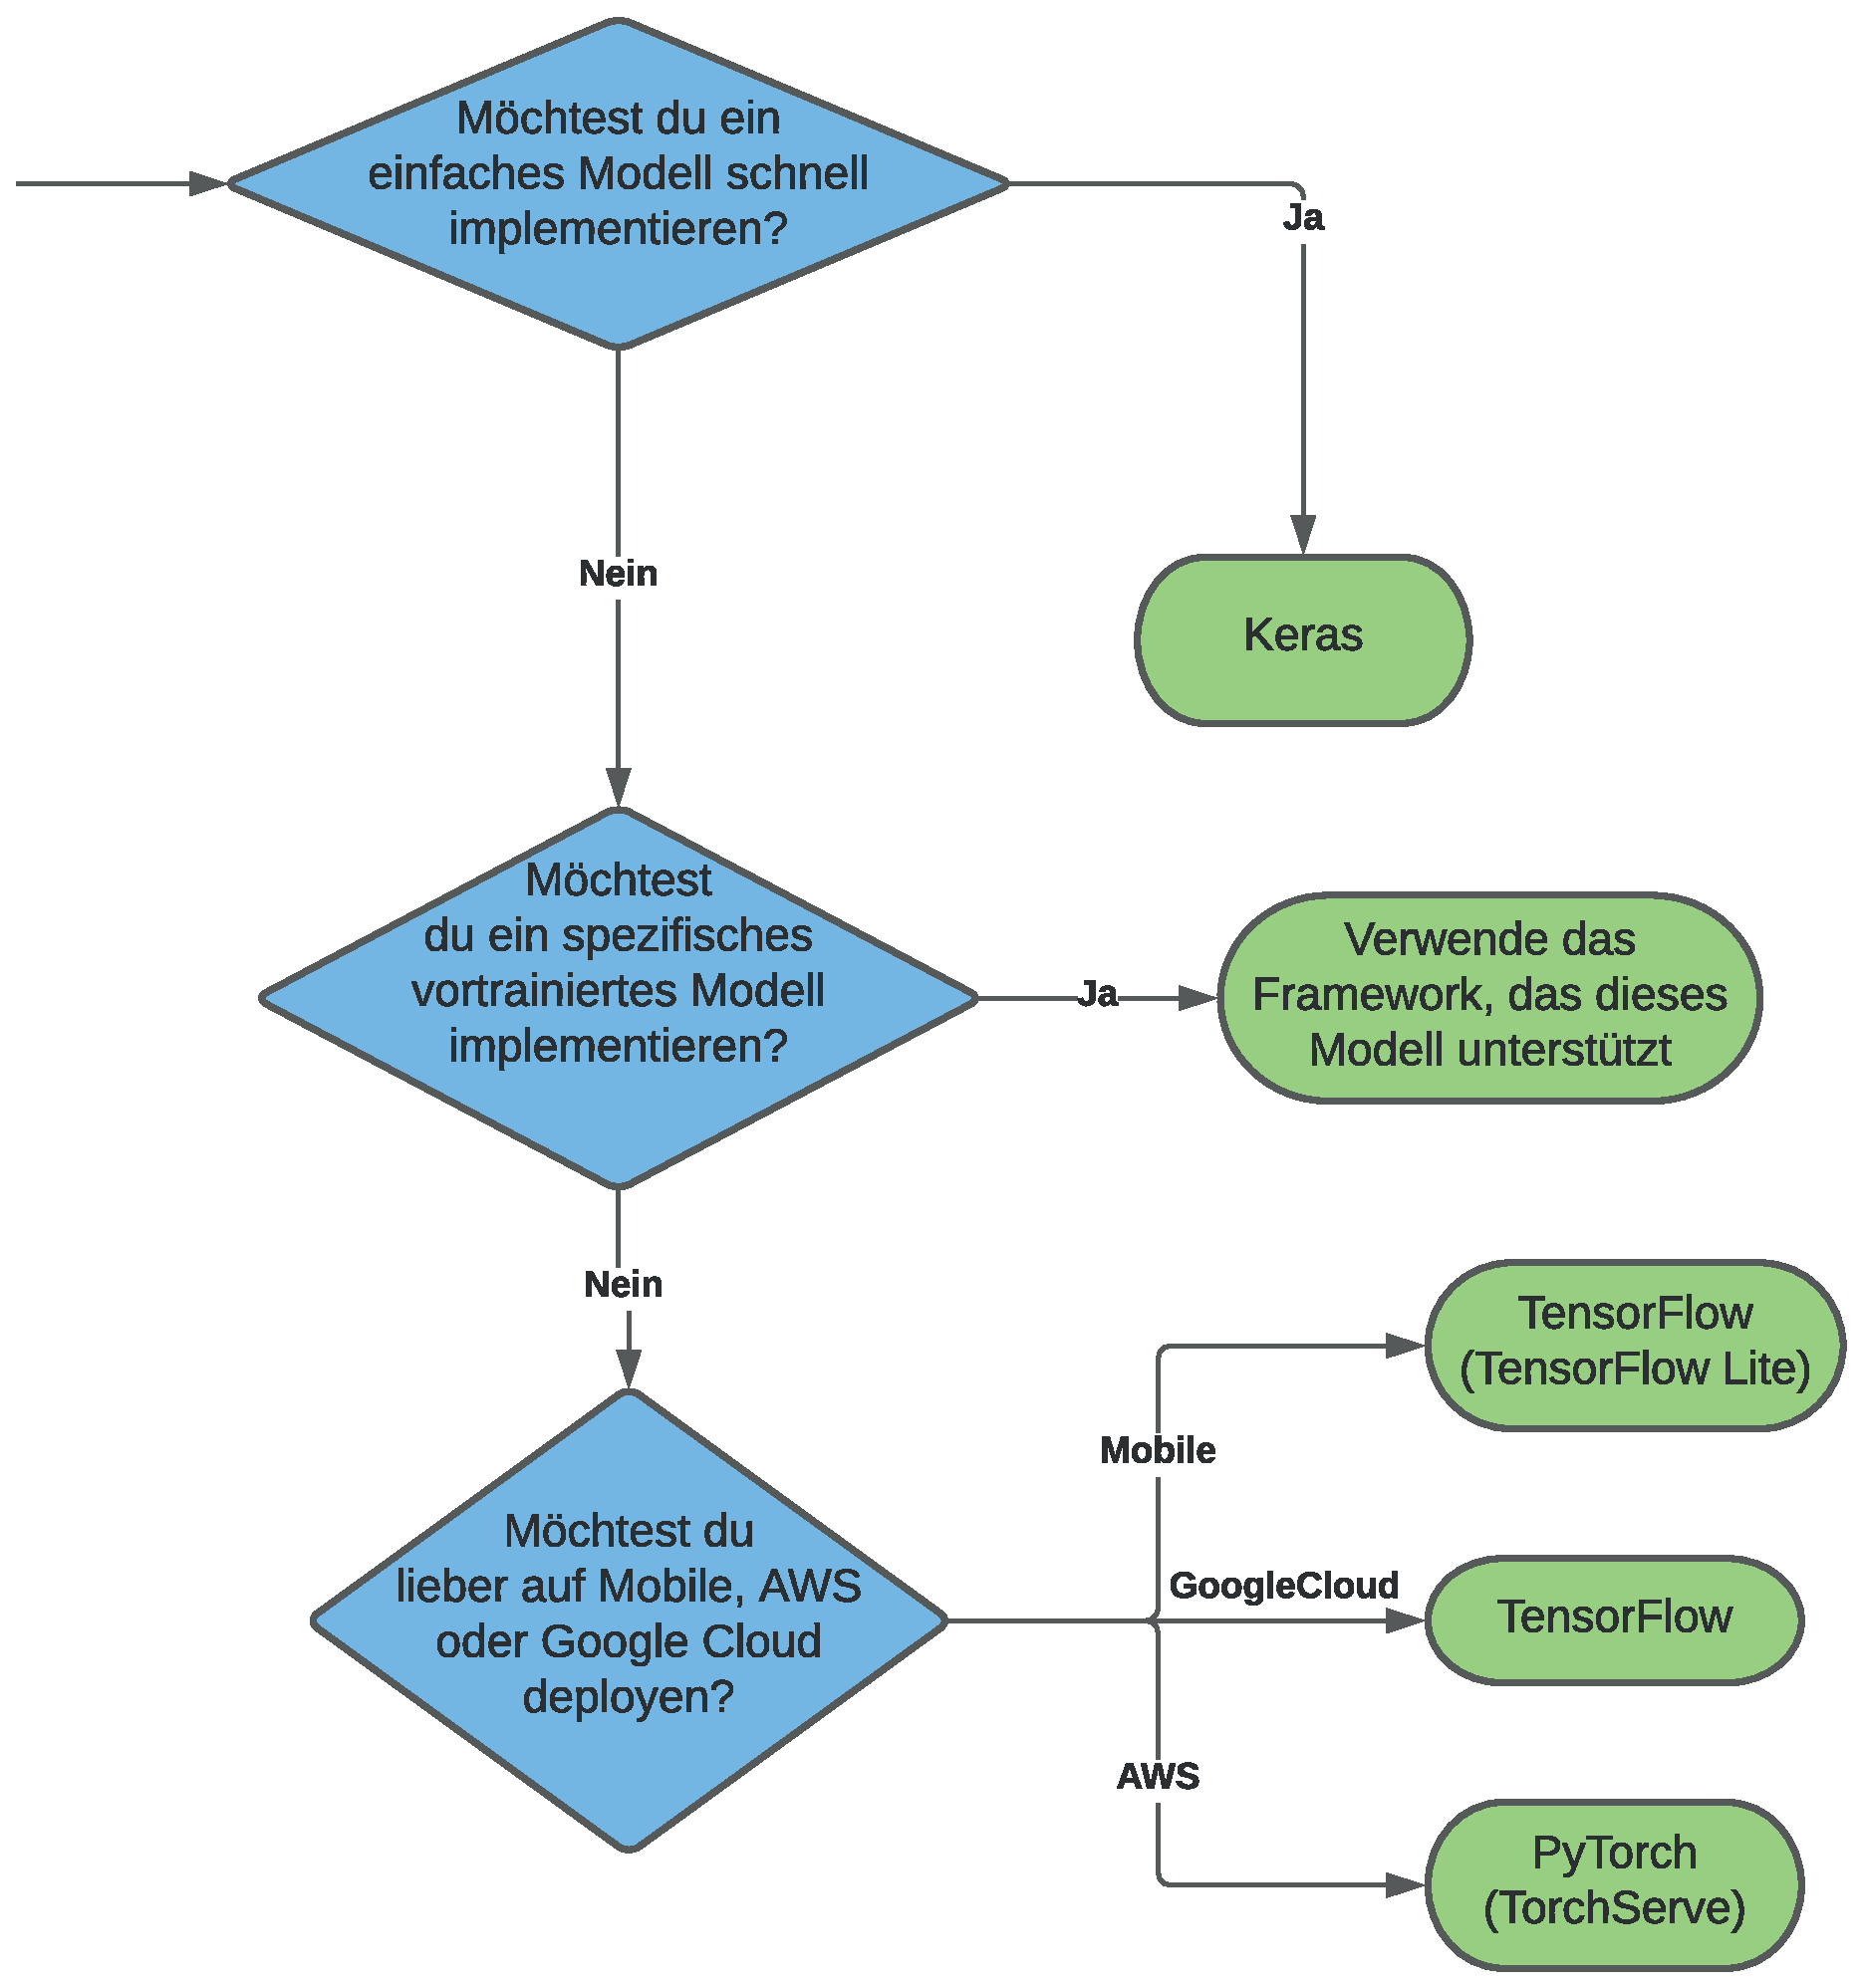
\includegraphics[width=.9\textwidth]{figures/decision-tree}
    \caption{Wann welches Framework verwenden?}
    \label{fig:decision-tree}
\end{figure}